% Options for packages loaded elsewhere
\PassOptionsToPackage{unicode}{hyperref}
\PassOptionsToPackage{hyphens}{url}
%
\documentclass[
  11pt,
]{article}
\usepackage{amsmath,amssymb}
\usepackage{lmodern}
\usepackage{setspace}
\usepackage{iftex}
\ifPDFTeX
  \usepackage[T1]{fontenc}
  \usepackage[utf8]{inputenc}
  \usepackage{textcomp} % provide euro and other symbols
\else % if luatex or xetex
  \usepackage{unicode-math}
  \defaultfontfeatures{Scale=MatchLowercase}
  \defaultfontfeatures[\rmfamily]{Ligatures=TeX,Scale=1}
\fi
% Use upquote if available, for straight quotes in verbatim environments
\IfFileExists{upquote.sty}{\usepackage{upquote}}{}
\IfFileExists{microtype.sty}{% use microtype if available
  \usepackage[]{microtype}
  \UseMicrotypeSet[protrusion]{basicmath} % disable protrusion for tt fonts
}{}
\makeatletter
\@ifundefined{KOMAClassName}{% if non-KOMA class
  \IfFileExists{parskip.sty}{%
    \usepackage{parskip}
  }{% else
    \setlength{\parindent}{0pt}
    \setlength{\parskip}{6pt plus 2pt minus 1pt}}
}{% if KOMA class
  \KOMAoptions{parskip=half}}
\makeatother
\usepackage{xcolor}
\usepackage[margin=1in]{geometry}
\usepackage{color}
\usepackage{fancyvrb}
\newcommand{\VerbBar}{|}
\newcommand{\VERB}{\Verb[commandchars=\\\{\}]}
\DefineVerbatimEnvironment{Highlighting}{Verbatim}{commandchars=\\\{\}}
% Add ',fontsize=\small' for more characters per line
\usepackage{framed}
\definecolor{shadecolor}{RGB}{248,248,248}
\newenvironment{Shaded}{\begin{snugshade}}{\end{snugshade}}
\newcommand{\AlertTok}[1]{\textcolor[rgb]{0.94,0.16,0.16}{#1}}
\newcommand{\AnnotationTok}[1]{\textcolor[rgb]{0.56,0.35,0.01}{\textbf{\textit{#1}}}}
\newcommand{\AttributeTok}[1]{\textcolor[rgb]{0.77,0.63,0.00}{#1}}
\newcommand{\BaseNTok}[1]{\textcolor[rgb]{0.00,0.00,0.81}{#1}}
\newcommand{\BuiltInTok}[1]{#1}
\newcommand{\CharTok}[1]{\textcolor[rgb]{0.31,0.60,0.02}{#1}}
\newcommand{\CommentTok}[1]{\textcolor[rgb]{0.56,0.35,0.01}{\textit{#1}}}
\newcommand{\CommentVarTok}[1]{\textcolor[rgb]{0.56,0.35,0.01}{\textbf{\textit{#1}}}}
\newcommand{\ConstantTok}[1]{\textcolor[rgb]{0.00,0.00,0.00}{#1}}
\newcommand{\ControlFlowTok}[1]{\textcolor[rgb]{0.13,0.29,0.53}{\textbf{#1}}}
\newcommand{\DataTypeTok}[1]{\textcolor[rgb]{0.13,0.29,0.53}{#1}}
\newcommand{\DecValTok}[1]{\textcolor[rgb]{0.00,0.00,0.81}{#1}}
\newcommand{\DocumentationTok}[1]{\textcolor[rgb]{0.56,0.35,0.01}{\textbf{\textit{#1}}}}
\newcommand{\ErrorTok}[1]{\textcolor[rgb]{0.64,0.00,0.00}{\textbf{#1}}}
\newcommand{\ExtensionTok}[1]{#1}
\newcommand{\FloatTok}[1]{\textcolor[rgb]{0.00,0.00,0.81}{#1}}
\newcommand{\FunctionTok}[1]{\textcolor[rgb]{0.00,0.00,0.00}{#1}}
\newcommand{\ImportTok}[1]{#1}
\newcommand{\InformationTok}[1]{\textcolor[rgb]{0.56,0.35,0.01}{\textbf{\textit{#1}}}}
\newcommand{\KeywordTok}[1]{\textcolor[rgb]{0.13,0.29,0.53}{\textbf{#1}}}
\newcommand{\NormalTok}[1]{#1}
\newcommand{\OperatorTok}[1]{\textcolor[rgb]{0.81,0.36,0.00}{\textbf{#1}}}
\newcommand{\OtherTok}[1]{\textcolor[rgb]{0.56,0.35,0.01}{#1}}
\newcommand{\PreprocessorTok}[1]{\textcolor[rgb]{0.56,0.35,0.01}{\textit{#1}}}
\newcommand{\RegionMarkerTok}[1]{#1}
\newcommand{\SpecialCharTok}[1]{\textcolor[rgb]{0.00,0.00,0.00}{#1}}
\newcommand{\SpecialStringTok}[1]{\textcolor[rgb]{0.31,0.60,0.02}{#1}}
\newcommand{\StringTok}[1]{\textcolor[rgb]{0.31,0.60,0.02}{#1}}
\newcommand{\VariableTok}[1]{\textcolor[rgb]{0.00,0.00,0.00}{#1}}
\newcommand{\VerbatimStringTok}[1]{\textcolor[rgb]{0.31,0.60,0.02}{#1}}
\newcommand{\WarningTok}[1]{\textcolor[rgb]{0.56,0.35,0.01}{\textbf{\textit{#1}}}}
\usepackage{longtable,booktabs,array}
\usepackage{calc} % for calculating minipage widths
% Correct order of tables after \paragraph or \subparagraph
\usepackage{etoolbox}
\makeatletter
\patchcmd\longtable{\par}{\if@noskipsec\mbox{}\fi\par}{}{}
\makeatother
% Allow footnotes in longtable head/foot
\IfFileExists{footnotehyper.sty}{\usepackage{footnotehyper}}{\usepackage{footnote}}
\makesavenoteenv{longtable}
\usepackage{graphicx}
\makeatletter
\def\maxwidth{\ifdim\Gin@nat@width>\linewidth\linewidth\else\Gin@nat@width\fi}
\def\maxheight{\ifdim\Gin@nat@height>\textheight\textheight\else\Gin@nat@height\fi}
\makeatother
% Scale images if necessary, so that they will not overflow the page
% margins by default, and it is still possible to overwrite the defaults
% using explicit options in \includegraphics[width, height, ...]{}
\setkeys{Gin}{width=\maxwidth,height=\maxheight,keepaspectratio}
% Set default figure placement to htbp
\makeatletter
\def\fps@figure{htbp}
\makeatother
\setlength{\emergencystretch}{3em} % prevent overfull lines
\providecommand{\tightlist}{%
  \setlength{\itemsep}{0pt}\setlength{\parskip}{0pt}}
\setcounter{secnumdepth}{-\maxdimen} % remove section numbering
\usepackage{float}
\floatplacement{figure}{ht}
\usepackage[section]{placeins}
\usepackage{longtable}
\usepackage{hyperref}
\hypersetup{colorlinks = true, linkcolor = blue, urlcolor = blue}
\widowpenalty10000
\clubpenalty10000
\usepackage[page,header]{appendix}
\usepackage{titletoc}
\usepackage{tocloft}
\usepackage{makecell}
\ifLuaTeX
  \usepackage{selnolig}  % disable illegal ligatures
\fi
\IfFileExists{bookmark.sty}{\usepackage{bookmark}}{\usepackage{hyperref}}
\IfFileExists{xurl.sty}{\usepackage{xurl}}{} % add URL line breaks if available
\urlstyle{same} % disable monospaced font for URLs
\hypersetup{
  pdftitle={Lecture: Bayesian Fundamentals},
  pdfauthor={Denis Cohen},
  hidelinks,
  pdfcreator={LaTeX via pandoc}}

\title{Lecture: Bayesian Fundamentals}
\author{Denis Cohen\footnote{Mannheim Centre for European Social Research, University of Mannheim, 68131 Mannheim, Germany. \href{mailto:denis.cohen@uni-mannheim.de}{\nolinkurl{denis.cohen@uni-mannheim.de}}.}}
\date{}

\begin{document}
\maketitle

\setstretch{1.5}
\hypertarget{bayesian-fundamentals}{%
\subsection{Bayesian Fundamentals}\label{bayesian-fundamentals}}

\hypertarget{the-punchline}{%
\subsubsection{The punchline}\label{the-punchline}}

In the Bayesian world the unobserved quantities are assigned distributional properties and, therefore, become random variables in the analysis.

These distributions come in two basic flavors. If the distribution of the unknown quantity is not conditioned on fixed data, it is called prior distribution because it describes knowledge prior to seeing data.

Alternatively, if the distribution is conditioned on data that we observe, it is clearly updated from the unconditioned state and, therefore, more informed. This distribution is called posterior distribution. {[}\ldots{]}

The punchline is this: All likelihood-based models are Bayesian models in which the prior distribution is an appropriately selected uniform prior, and as the size of the data gets large they are identical given any finite appropriate prior. So such empirical researchers are really Bayesian; they just do not know it yet.

\href{https://academic.oup.com/jpart/article/23/2/457/1003493}{Gill, J., \& Witko, C. (2013). Bayesian analytical methods: A methodological prescription for public administration. Journal of Public Administration Research and Theory, 23(2), 457--494.}

\hypertarget{likelihood-function}{%
\subsubsection{Likelihood function}\label{likelihood-function}}

\begin{itemize}
\tightlist
\item
  Specification of a pdf or pmf: \(p(\mathbf{y}|\theta)\).
\item
  Also called the data generating process (or the generative model) for \(y\).
\item
  Logical inversion: ``Which unknown \(\theta\) most likely produces the known \(\mathbf{y}\)?'' \(\rightarrow\) \(L(\theta | \mathbf{y})\).
\item
  The notational distinction between \(p(\mathbf{y}|\theta)\) and \(L(\theta | \mathbf{y})\) is purely conceptual. \(p(\mathbf{y}|\theta) = L(\theta | \mathbf{y})\).
\item
  We will use \(p(\mathbf{y}|\theta)\).
\item
  Note that the likelihood function multiplies densities across \emph{all} observations; e.g., a normal likelihood function is given by:
\end{itemize}

\[p(\mathbf{y}|\mu, \sigma) = \prod_{i=1}^{N} \frac{1}{\sigma \sqrt{2 \pi}} \exp\left(- 0.5 \left( (y_i - \mu_i)^2 / \sigma \right) \right)\]

\begin{itemize}
\tightlist
\item
  This is what we mean mathematically when we use the shorthand

  \begin{itemize}
  \tightlist
  \item
    \(\mathbf{y} \sim \text{N}(\mu, \sigma)\) or
  \item
    \(y_i \sim \text{N}(\mu_i, \sigma) \text{ for all } i=1,...N\).
  \end{itemize}
\end{itemize}

\hypertarget{prior-distribution}{%
\subsubsection{Prior distribution}\label{prior-distribution}}

\begin{itemize}
\tightlist
\item
  A distributional characterization of our belief about an unknown quantity (i.e., a parameter) prior to seeing the data: \(p(\theta)\)
\item
  This includes statements about \emph{family}, \emph{support}, and \emph{density}.

  \begin{itemize}
  \tightlist
  \item
    \emph{Family}: A pdf (continuous parameters) or pmf (discrete parameters) that can plausibly generate the parameter values.
  \item
    \emph{Support}: Some parameters have constrained support: Probability parameters must be inside \([0, 1]\); variance parameters must be \(\geq 0\).
  \item
    \emph{Density}: A distributional characterization which values of the parameter we think are more or less likely to observe.
  \end{itemize}
\item
  The prior distribution can be

  \begin{itemize}
  \tightlist
  \item
    flat (i.e., uniformly distributed over the supported range -- often improper)
  \item
    purposefully very vague, and thus, rather uninformative
  \item
    weakly informative
  \item
    specific and substantively informed (e.g., by previous research or expert assessment)
  \end{itemize}
\end{itemize}

\hypertarget{posterior-distribution}{%
\subsubsection{Posterior distribution}\label{posterior-distribution}}

\begin{itemize}
\tightlist
\item
  Updating our distributional belief about \(\theta\) given the data, \(\mathbf{y}\): \(p(\theta | \mathbf{y})\)
\item
  Follows the proportional version of \href{https://en.wikipedia.org/wiki/Bayes\%27_theorem}{Bayes' Law}: \(p(\theta | \mathbf{y}) \propto p(\theta) \times p(\mathbf{y}|\theta)\)
\item
  Yields a weighthed combination of likelihood and prior
\item
  The prior pulls the posterior density toward the center of gravity of the prior distribution
\item
  As the data grows large, the likelihood becomes more influential:

  \begin{itemize}
  \tightlist
  \item
    one factor for \(p(\theta)\), \(N\) factors for \(p(y_i|\theta_i)\)
  \item
    we will see this analytically and using simulations later on
  \end{itemize}
\end{itemize}

\hypertarget{coin-flip-experiment}{%
\subsection{Coin flip experiment}\label{coin-flip-experiment}}

\hypertarget{the-experiment}{%
\subsubsection{The experiment}\label{the-experiment}}

Suppose we flip a coin up to \(N\) times:

\begin{itemize}
\tightlist
\item
  The fairness of a coin can be expressed through a \emph{probability parameter}, \(\pi\), that governs the probability that a coin flip produces heads (1) has opposed to tails (0)
\item
  We start out with the belief that the coin is fair -- that is, we consider it more probable that the coin is fair (\(\pi \approx 0.5\)) and less probable that it systematically over-produces either heads or tails
\item
  Unbeknownst to us, the coin is far from fair -- it is 4 times as likely to produce heads as it is to produce tails (that is, \(\pi=0.8\))
\item
  We slowly learn about this in the process of flipping the coin and keeping score of the number of flips \(n\) and the number of heads \(k\)\ldots{}
\end{itemize}

\hypertarget{analytical-form-prior-distribution}{%
\subsubsection{Analytical form: Prior distribution}\label{analytical-form-prior-distribution}}

\begin{itemize}
\tightlist
\item
  The \emph{beta distribution} is a suitable candidate for characterizing our prior beliefs: \(\pi \sim \text{beta}(a,b)\)
\item
  Characterized by two shape parameters, \(a\) and \(b\)
\item
  \(a\) and \(b\) are \emph{hyperparameters}: Known (or chosen) parameters that characterize a prior distribution.
\item
  Constrained support: \(\pi \in [0, 1]\)
\item
  pdf: \(p(\pi) = \frac{\pi^{a-1} (1- \pi)^{b-1}}{\text{B}(a, b)}\)
\end{itemize}

\begin{center}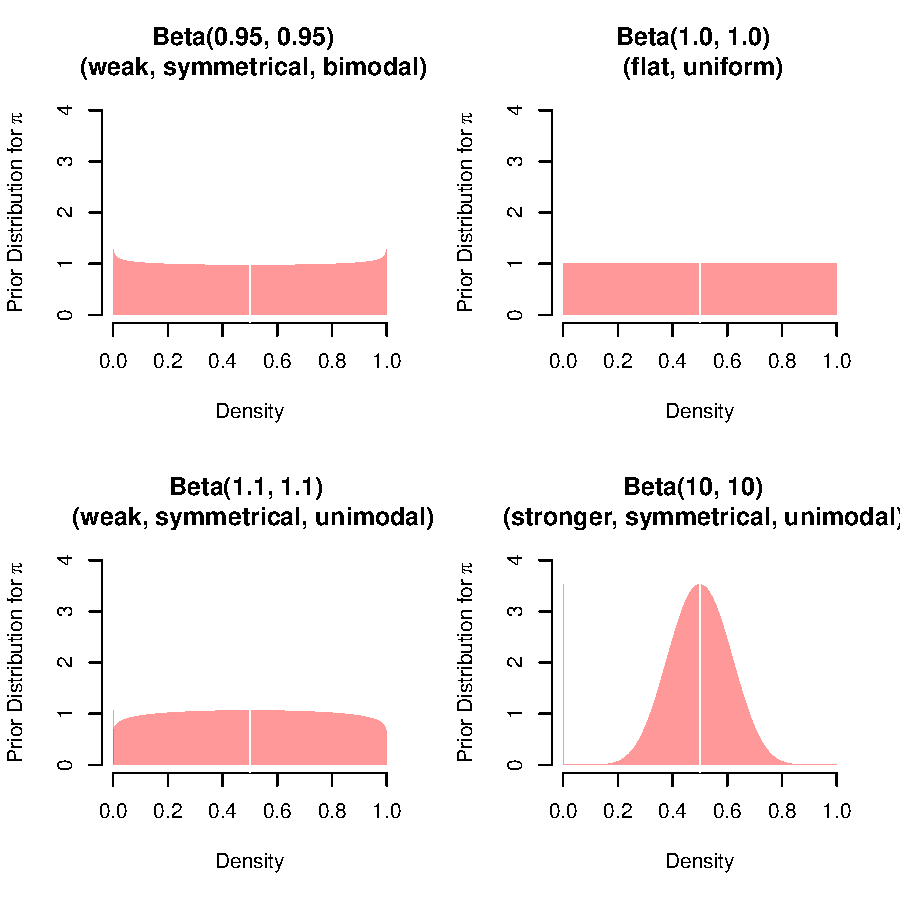
\includegraphics{03-lec_files/figure-latex/beta-1} \end{center}

\hypertarget{analytical-form-likelihood}{%
\subsubsection{Analytical form: Likelihood}\label{analytical-form-likelihood}}

\begin{itemize}
\tightlist
\item
  Flipping one and the same coin \(n\) times is a series of Bernoulli trials
\item
  The \emph{binomial distribution} describes the corresponding data generating process: \(k \sim \text{Binomial}(n, \pi)\)
\item
  pmf: \(p(k|n, \pi) = {n \choose k} \pi^k (1-\pi)^{(n-k)}\)
\end{itemize}

\hypertarget{analytical-form-posterior-distribution}{%
\subsubsection{Analytical form: Posterior distribution}\label{analytical-form-posterior-distribution}}

Remember: \[p(\theta | \mathbf{y}) \propto p(\theta) \times p(\mathbf{y}|\theta)\]

So what does this mean in the present example?

\[\begin{split}p(\pi|n,k) & \propto p(\pi) \times p(k|n, \pi) \\
 p(\pi|n,k) & \propto \frac{\pi^{a-1} (1- \pi)^{b-1}}{\text{B}(a, b)} \times {n \choose k} \pi^k (1-\pi)^{(n-k)}\end{split}\]

Note that since we use the proportional version of Bayes' Law (i.e., we do not stipulate exact equality), we can drop any constant terms that do not involve our parameter of interest, \(\pi\):

\[\begin{split}p(\pi|n,k) & \propto \pi^{a-1} (1- \pi)^{b-1} \times \pi^k (1-\pi)^{(n-k)}\end{split}\]
The rest, then, is easy: Following the rules of exponentiation, we add exponents for identical bases. This gives us our posterior distribution for \(\pi\):

\[\begin{split}p(\pi|n,k) & \propto \pi^{a+k-1} (1- \pi)^{b+n-k-1}\end{split}\]
As you see, our posterior has the exact same form as our prior. It is a beta distribution with updated parameters

\begin{itemize}
\tightlist
\item
  \(a^{\prime} = a+k-1\)
\item
  \(b^{\prime} = b+n-k-1\)
\end{itemize}

This property is called \emph{conjugacy}: Prior and posterior are of the same family.

Now, take a moment to think about our analytical solution for the updated parameter:

\begin{itemize}
\tightlist
\item
  What does it take for the data to dominate the prior?
\item
  What if the prior is weak (e.g., \(\pi \sim \text{beta}(1,1)\))?
\item
  What if the prior is strong (e.g., \(\pi \sim \text{beta}(100,100)\))?
\end{itemize}

\hypertarget{simulation}{%
\subsubsection{Simulation}\label{simulation}}

\hypertarget{prior-distribution-1}{%
\paragraph{Prior distribution}\label{prior-distribution-1}}

Code: Defining and plotting the prior distribution

\begin{Shaded}
\begin{Highlighting}[]
\NormalTok{len\_pi }\OtherTok{\textless{}{-}}\NormalTok{ 1001L                      }\DocumentationTok{\#\#\# number of candidate values for pi}
\NormalTok{pi }\OtherTok{\textless{}{-}} \FunctionTok{seq}\NormalTok{(}\DecValTok{0}\NormalTok{, }\DecValTok{1}\NormalTok{, }\AttributeTok{length.out =}\NormalTok{ len\_pi) }\DocumentationTok{\#\#\# candidate values for pi}
\NormalTok{a }\OtherTok{\textless{}{-}}\NormalTok{ b }\OtherTok{\textless{}{-}} \DecValTok{5}                          \DocumentationTok{\#\#\# hyperparameters}
\NormalTok{prior }\OtherTok{\textless{}{-}} \FunctionTok{dbeta}\NormalTok{(pi, a, b)             }\DocumentationTok{\#\#\# prior distribution}

\DocumentationTok{\#\# Plot}
\FunctionTok{plot}\NormalTok{(                                }\DocumentationTok{\#\#\# set up empty plot, specify labels}
\NormalTok{  pi, prior,}
  \AttributeTok{type =} \StringTok{\textquotesingle{}n\textquotesingle{}}\NormalTok{,}
  \AttributeTok{xlab =} \StringTok{"Density"}\NormalTok{,}
  \AttributeTok{ylab =} \FunctionTok{expression}\NormalTok{(}\FunctionTok{paste}\NormalTok{(}\StringTok{"Prior Distribution for "}\NormalTok{, pi))}
\NormalTok{)}
\FunctionTok{polygon}\NormalTok{(                             }\DocumentationTok{\#\#\# draw density distribution}
  \FunctionTok{c}\NormalTok{(}\FunctionTok{rep}\NormalTok{(}\DecValTok{0}\NormalTok{, }\FunctionTok{length}\NormalTok{(pi)), pi),}
  \FunctionTok{c}\NormalTok{(prior, }\FunctionTok{rev}\NormalTok{(prior)),}
  \AttributeTok{col =} \FunctionTok{adjustcolor}\NormalTok{(}\StringTok{\textquotesingle{}red\textquotesingle{}}\NormalTok{, }\AttributeTok{alpha.f =}\NormalTok{ .}\DecValTok{4}\NormalTok{),}
  \AttributeTok{border =} \ConstantTok{NA}
\NormalTok{)}
\FunctionTok{abline}\NormalTok{(                              }\DocumentationTok{\#\#\# add vertical at pi = 0.5 }
  \AttributeTok{v =}\NormalTok{ .}\DecValTok{5}\NormalTok{,}
  \AttributeTok{col =} \StringTok{\textquotesingle{}white\textquotesingle{}}
\NormalTok{)}
\end{Highlighting}
\end{Shaded}

\begin{center}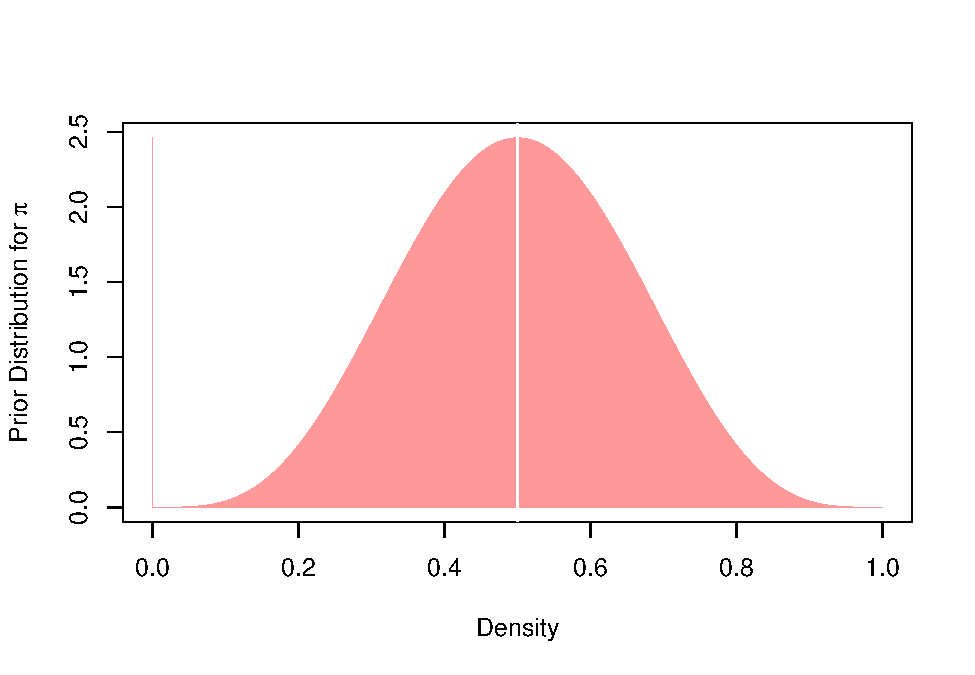
\includegraphics[width=0.75\linewidth]{03-lec_files/figure-latex/coin-sim0-print-1} \end{center}

\hypertarget{posterior-distribution-1}{%
\paragraph{Posterior distribution}\label{posterior-distribution-1}}

Code: Simulating the experiment

\begin{Shaded}
\begin{Highlighting}[]
\FunctionTok{set.seed}\NormalTok{(}\DecValTok{20210329}\NormalTok{)                   }\DocumentationTok{\#\#\# set seed for replicability}
\NormalTok{len\_pi }\OtherTok{\textless{}{-}}\NormalTok{ 1001L                      }\DocumentationTok{\#\#\# number of candidate values for pi}
\NormalTok{pi }\OtherTok{\textless{}{-}} \FunctionTok{seq}\NormalTok{(}\DecValTok{0}\NormalTok{, }\DecValTok{1}\NormalTok{, }\AttributeTok{length.out =}\NormalTok{ len\_pi) }\DocumentationTok{\#\#\# candidate values for pi}
\NormalTok{a }\OtherTok{\textless{}{-}}\NormalTok{ b }\OtherTok{\textless{}{-}} \DecValTok{5}                          \DocumentationTok{\#\#\# hyperparameters}
\NormalTok{n }\OtherTok{\textless{}{-}} \DecValTok{300}                             \DocumentationTok{\#\#\# num. of coin flips}
\NormalTok{pi\_true }\OtherTok{\textless{}{-}}\NormalTok{ .}\DecValTok{8}                        \DocumentationTok{\#\#\# true parameter}
\NormalTok{data }\OtherTok{\textless{}{-}} \FunctionTok{rbinom}\NormalTok{(n, }\DecValTok{1}\NormalTok{, pi\_true)        }\DocumentationTok{\#\#\# n coin flips}
\NormalTok{posterior }\OtherTok{\textless{}{-}} \FunctionTok{matrix}\NormalTok{(}\ConstantTok{NA}\NormalTok{, 3L, n)       }\DocumentationTok{\#\#\# matrix container for posterior}

\ControlFlowTok{for}\NormalTok{ (i }\ControlFlowTok{in} \FunctionTok{seq\_len}\NormalTok{(n)) \{    }
\NormalTok{  current\_sequence }\OtherTok{\textless{}{-}}\NormalTok{ data[}\DecValTok{1}\SpecialCharTok{:}\NormalTok{i]      }\DocumentationTok{\#\#\# sequence up until ith draw}
\NormalTok{  k }\OtherTok{\textless{}{-}} \FunctionTok{sum}\NormalTok{(current\_sequence)         }\DocumentationTok{\#\#\# number of heads in current sequence}
  
  \DocumentationTok{\#\#\#\#\# Updating}
\NormalTok{  a\_prime }\OtherTok{\textless{}{-}}\NormalTok{ a }\SpecialCharTok{+}\NormalTok{ k               }
\NormalTok{  b\_prime }\OtherTok{\textless{}{-}}\NormalTok{ b }\SpecialCharTok{+}\NormalTok{ i }\SpecialCharTok{{-}}\NormalTok{ k}
  
  \DocumentationTok{\#\#\# Analytical means and credible intervals}
\NormalTok{  posterior[}\DecValTok{1}\NormalTok{, i] }\OtherTok{\textless{}{-}}\NormalTok{ a\_prime }\SpecialCharTok{/}\NormalTok{ (a\_prime }\SpecialCharTok{+}\NormalTok{ b\_prime)}
\NormalTok{  posterior[}\DecValTok{2}\NormalTok{, i] }\OtherTok{\textless{}{-}} \FunctionTok{qbeta}\NormalTok{(}\FloatTok{0.025}\NormalTok{, a\_prime, b\_prime)}
\NormalTok{  posterior[}\DecValTok{3}\NormalTok{, i] }\OtherTok{\textless{}{-}} \FunctionTok{qbeta}\NormalTok{(}\FloatTok{0.975}\NormalTok{, a\_prime, b\_prime)}
\NormalTok{\}}

\DocumentationTok{\#\# Plot}
\FunctionTok{plot}\NormalTok{(                                }\DocumentationTok{\#\#\# set up empty plot with labels}
  \DecValTok{1}\SpecialCharTok{:}\NormalTok{n, }\DecValTok{1}\SpecialCharTok{:}\NormalTok{n,}
  \AttributeTok{type =} \StringTok{\textquotesingle{}n\textquotesingle{}}\NormalTok{,}
  \AttributeTok{xlab =} \StringTok{"Number of Coin Flips"}\NormalTok{,}
  \AttributeTok{ylab =} \FunctionTok{expression}\NormalTok{(}\FunctionTok{paste}\NormalTok{(}\StringTok{"Posterior Means of "}\NormalTok{,}
\NormalTok{                          pi,}
                          \AttributeTok{sep =} \StringTok{" "}\NormalTok{)), }
  \AttributeTok{ylim =} \FunctionTok{c}\NormalTok{(}\DecValTok{0}\NormalTok{, }\DecValTok{1}\NormalTok{),}
  \AttributeTok{xlim =} \FunctionTok{c}\NormalTok{(}\DecValTok{1}\NormalTok{, n)}
\NormalTok{)}
\FunctionTok{abline}\NormalTok{(                              }\DocumentationTok{\#\#\# reference line for the true pi}
  \AttributeTok{h =} \FunctionTok{c}\NormalTok{(.}\DecValTok{5}\NormalTok{, .}\DecValTok{8}\NormalTok{),}
  \AttributeTok{col =} \StringTok{"gray80"}
\NormalTok{)}
\FunctionTok{rect}\NormalTok{(}\SpecialCharTok{{-}}\NormalTok{.}\DecValTok{5}\NormalTok{, }\FunctionTok{qbeta}\NormalTok{(}\FloatTok{0.025}\NormalTok{, }\DecValTok{5}\NormalTok{, }\DecValTok{5}\NormalTok{),        }\DocumentationTok{\#\#\# prior mean + interval at i = 0}
     \FloatTok{0.5}\NormalTok{, }\FunctionTok{qbeta}\NormalTok{(}\FloatTok{0.975}\NormalTok{, }\DecValTok{5}\NormalTok{, }\DecValTok{5}\NormalTok{),}
     \AttributeTok{col =} \FunctionTok{adjustcolor}\NormalTok{(}\StringTok{\textquotesingle{}red\textquotesingle{}}\NormalTok{, .}\DecValTok{4}\NormalTok{),}
     \AttributeTok{border =} \FunctionTok{adjustcolor}\NormalTok{(}\StringTok{\textquotesingle{}red\textquotesingle{}}\NormalTok{, .}\DecValTok{2}\NormalTok{))}
\FunctionTok{segments}\NormalTok{(}\SpecialCharTok{{-}}\NormalTok{.}\DecValTok{5}\NormalTok{, .}\DecValTok{5}\NormalTok{,}
         \FloatTok{0.5}\NormalTok{, .}\DecValTok{5}\NormalTok{,}
         \AttributeTok{col =} \FunctionTok{adjustcolor}\NormalTok{(}\StringTok{\textquotesingle{}red\textquotesingle{}}\NormalTok{, .}\DecValTok{9}\NormalTok{),}
         \AttributeTok{lwd =} \FloatTok{1.5}\NormalTok{)}
\FunctionTok{polygon}\NormalTok{(                             }\DocumentationTok{\#\#\# posterior means + intervals}
  \FunctionTok{c}\NormalTok{(}\FunctionTok{seq\_len}\NormalTok{(n), }\FunctionTok{rev}\NormalTok{(}\FunctionTok{seq\_len}\NormalTok{(n))),}
  \FunctionTok{c}\NormalTok{(posterior[}\DecValTok{2}\NormalTok{, ], }\FunctionTok{rev}\NormalTok{(posterior[}\DecValTok{3}\NormalTok{, ])),}
  \AttributeTok{col =} \FunctionTok{adjustcolor}\NormalTok{(}\StringTok{\textquotesingle{}blue\textquotesingle{}}\NormalTok{, .}\DecValTok{4}\NormalTok{),}
  \AttributeTok{border =} \FunctionTok{adjustcolor}\NormalTok{(}\StringTok{\textquotesingle{}blue\textquotesingle{}}\NormalTok{, .}\DecValTok{2}\NormalTok{)}
\NormalTok{)}
\FunctionTok{lines}\NormalTok{(}
  \FunctionTok{seq\_len}\NormalTok{(n),}
\NormalTok{  posterior[}\DecValTok{1}\NormalTok{, ],}
  \AttributeTok{col =} \FunctionTok{adjustcolor}\NormalTok{(}\StringTok{\textquotesingle{}blue\textquotesingle{}}\NormalTok{, .}\DecValTok{9}\NormalTok{),}
  \AttributeTok{lwd =} \FloatTok{1.5}
\NormalTok{)}
\end{Highlighting}
\end{Shaded}

\begin{center}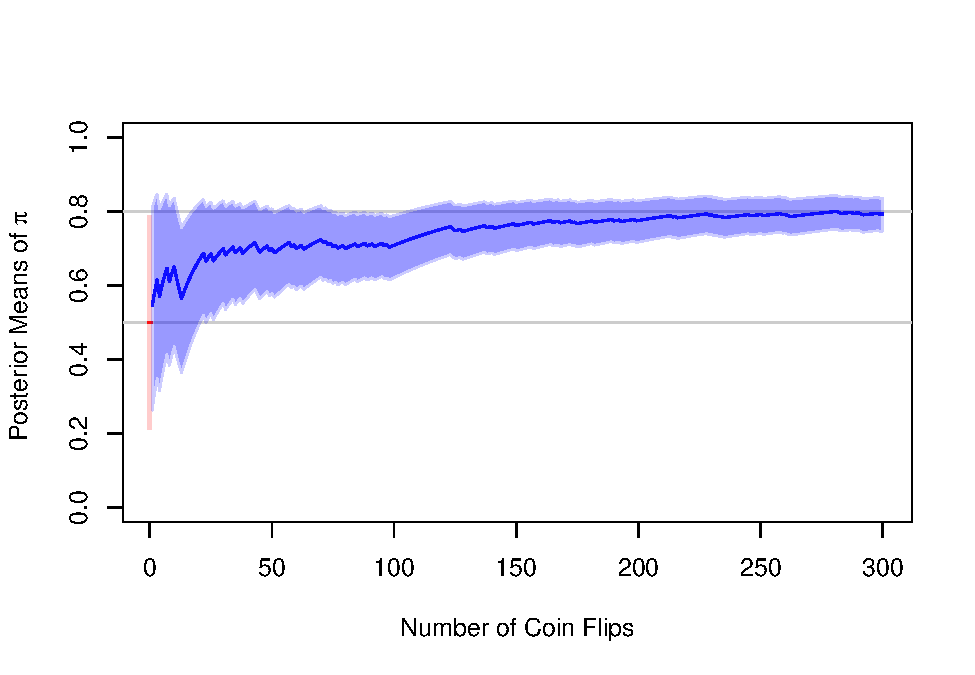
\includegraphics[width=0.75\linewidth]{03-lec_files/figure-latex/coin-sim2-1} \end{center}

\emph{Note:} After 300 coin flips, we have observed 241 heads, which is a proportion of 0.803. The posterior median is 0.794; the 95\% credible interval is {[}0.747, 0.837{]}.

\hypertarget{mcmc-algorithms}{%
\subsection{MCMC algorithms}\label{mcmc-algorithms}}

\hypertarget{analytical-classical-bayesian-inference}{%
\subsubsection{Analytical (classical) Bayesian inference}\label{analytical-classical-bayesian-inference}}

\begin{itemize}
\tightlist
\item
  As you may have noticed: Our coin flip example did \emph{not} involve \emph{any} numerical estimation algorithms.
\item
  We simply observed the data, applied Bayes' Law, and analytically updated our parameters.
\item
  This allowed us to retrieve a distributional characterization of our parameter of interest at each iteration of the coin flip series.
\item
  The reasons why we could do this with ease is that this simple Binomial problem involved a single parameter \(\pi\); i.e, we were dealing with a uni-dimensional \emph{parameter space}.
\end{itemize}

\hypertarget{the-limits-of-analytical-bayesian-inference}{%
\subsubsection{The limits of analytical Bayesian inference}\label{the-limits-of-analytical-bayesian-inference}}

\begin{itemize}
\tightlist
\item
  Even in only slightly more intricate applications, Bayesian inference involves finding a \emph{joint} posterior for \emph{all} parameters in a model, i.e., finding a \emph{multi-dimensional} parameter space.
\item
  Inference on single parameters from a joint multi-dimensional parameter space requires that we retrieve the marginal posterior distribution from the joint posterior distribution.
\item
  Marginalizing the joint multidimensional posterior distribution w.r.t. to a given a parameter gives the posterior distribution for that parameter. This requires \emph{integrating} out all other parameters.
\item
  For instance, when our joint posterior in a three-dimensional parameter space is \(p(\alpha,\beta, \gamma)\), we need to obtain each marginal posterior akin to \(p(\alpha) = \int_{\beta} \int_{\gamma} p(\alpha,\beta, \gamma) d\beta d\gamma\)
\item
  For complex multi-dimensional posterior distributions, finding analytical solutions through integration becomes cumbersome, if not outright impossible.
\end{itemize}

\hypertarget{numerical-approximation-via-mcmc}{%
\subsubsection{Numerical approximation via MCMC}\label{numerical-approximation-via-mcmc}}

That's where numerical approximation through Markov Chain Monte Carlo (MCMC) algorithms comes in:

\begin{itemize}
\tightlist
\item
  MCMC are iterative computational processes that explore and describe a posterior distribution.
\item
  Developed in the 1980s and popularized in the 1990s, MCMC algorithms quickly eliminated the need for analytical marginalizations of single parameters from joint multi-dimensional posteriors.
\item
  The core idea:

  \begin{itemize}
  \tightlist
  \item
    \emph{Markov Chains} wander through, and take samples from, the parameter space.Following an initial warmup period, the Markov Chains will converge to high-density regions of the underlying posterior distribution (ergodicity).
  \item
    The proportion of ``steps'' in a given region of multidimensional parameter space gives a stochastic simulation of the posterior probability density.
  \item
    This yields a numerical approximation of the underlying posterior distribution, much like Monte Carlo simulations of MLE parameters yield numerical approximations of the underlying sampling distribution.
  \end{itemize}
\end{itemize}

\hypertarget{some-mcmc-algorithms}{%
\subsubsection{(Some) MCMC Algorithms}\label{some-mcmc-algorithms}}

\begin{enumerate}
\def\labelenumi{\arabic{enumi}.}
\tightlist
\item
  \textbf{Gibbs}: Draws iteratively and alternatively from the conditional conjugate distribution of each parameter.
\item
  \textbf{Metropolis-Hastings}: Considers a single multidimensional move on each iteration depending on the quality of the proposed candidate draw.
\item
  \textbf{Hamiltonian Monte Carlo (HMC)}, used in Stan:
\end{enumerate}

The Hamiltonian Monte Carlo algorithm starts at a specified initial set of parameters \(\theta\); in Stan, this value is either user-specified or generated randomly. Then, for a given number of iterations, a new momentum vector is sampled and the current value of the parameter \(\theta\) is updated using the leapfrog integrator with discretization time \(\epsilon\) and number of steps \(L\) according to the Hamiltonian dynamics. Then a Metropolis acceptance step is applied, and a decision is made whether to update to the new state \((\theta^{\ast},\rho{\ast})\) or keep the existing state.

Source: \href{https://mc-stan.org/docs/2_19/reference-manual/hamiltonian-monte-carlo.html}{Stan Reference Manual, Section 14.1}

\hypertarget{implementing-a-gibbs-sampler}{%
\subsection{Implementing a Gibbs sampler}\label{implementing-a-gibbs-sampler}}

\hypertarget{in-a-nutshell}{%
\subsubsection{In a nutshell}\label{in-a-nutshell}}

\begin{itemize}
\tightlist
\item
  We want to perform inference on a variable \(y\), of which we have \(N\) observations.
\item
  We stipulate that the data-generating process that produces \(y\) is normal: \(\mathbf{y} \sim \text{N}(\mu, \sigma^2)\). This yields a two-dimensional parameter space.
\item
  For reasons of convenience, we parameterize the variance of this normal distribution in terms of its precision \(\tau = \frac{1}{\sigma^2}\), not in terms of its standard deviation or variance.
\item
  Note, however, that \texttt{rnorm()} in R uses the standard deviation, which is \texttt{sqrt(1\ /\ tau)}.
\item
  We will use a \emph{Gibbs sampler}. Remember that Gibbs draws iteratively and alternatively from the conditional conjugate distribution of each parameter.
\item
  We thus need some analytical preliminaries: Namely, analytical forms for the posterior distributions of the two parameters from whose marginal posteriors we would like to sample.
\item
  This will \emph{not} involve marginalizing out the ``unwanted'' parameters; instead, we will derive the posteriors of \(\mu\) and \(\tau\) as conditional functions of \(\tau\) and \(\mu\), respectively
\end{itemize}

\hypertarget{application}{%
\subsubsection{Application}\label{application}}

\begin{itemize}
\tightlist
\item
  Specifically, we will focus on the variable \texttt{sup\_afd} from the data set \texttt{gles}.
\item
  Let's pretend our prior belief is completely naive:

  \begin{itemize}
  \tightlist
  \item
    We don't know how (un)popular the AfD is in the German electorate
  \item
    But we know that individual support is measured on a -5 to 5 scale
  \item
    Our prior belief for \(\mu\) should thus be agnostic as to whether people like or dislike the AfD and sufficiently vague to allow for the possibility that we may be wrong: \(\mu \sim \text{N}(\theta = 0, \omega^{-1} = 10)\) (mean \(\theta\) and precision \(\omega\) are hyperparameters for the prior of \(\mu\))
  \item
    Our prior belief for \(\tau\) will also be vague: \(\tau \sim \Gamma(\alpha = 20, \beta = 200)\) (shape \(\alpha\) and rate \(\beta\) are hyperparameters for the prior of \(\tau\))
  \item
    We have no prior belief about the dependence of both parameters and hence specify independent prior distributions
  \end{itemize}
\end{itemize}

\hypertarget{analytical-preliminaries-mu}{%
\subsubsection{\texorpdfstring{Analytical preliminaries: \(\mu\)}{Analytical preliminaries: \textbackslash mu}}\label{analytical-preliminaries-mu}}

Our prior belief is that \(\mu\) is distributed normal with mean \(\theta = 0\) and precision \(\omega = .1\):

\[\mu \sim \text{N}(0, 10)\]

The prior pdf is given by:

\[
p(\mu | \theta, \omega) = \sqrt{\frac{\omega}{2 \pi}} \exp \left (-\frac{\omega (\mu - \theta)^2}{2} \right)
\]

while the likelihood for the data \(\mathbf{y}\) is given by

\[
p(\mathbf{y} | \mu, \tau) = \prod_{i}^{N} \sqrt{\frac{\tau}{2\pi}} \exp\left(-\frac{\tau(y_i-\mu)^2}{2} \right)
\]

Multiplying prior and likelihood and performing some algebraic transformations, we see that our conditional posterior density will be

\[
p(\mu | \theta, \omega, \tau, \mathbf{y}) \propto \exp \left(-\frac{\omega + N \tau}{2}  \left(\mu - \frac{\omega \theta + N \tau \bar{y}}{\omega + N \tau}\right)^2 \right)
\]

We recognize this as the normal pdf with updated mean parameter \(\theta^{\ast} = \frac{\omega \theta + N \tau \bar{y}}{\omega + N \tau}\) and updated precision parameter \(\omega^{\ast} = \omega + N \tau\).

This gives us the required analytical solutions for the normal parameters that characterize the posterior density of \(\mu\).

\hypertarget{analytical-preliminaries-tau}{%
\subsubsection{\texorpdfstring{Analytical preliminaries: \(\tau\)}{Analytical preliminaries: \textbackslash tau}}\label{analytical-preliminaries-tau}}

Furthermore, for our prior knowledge about the precision, we assume that \(\tau\) is Gamma-distributed with shape \(\alpha=20\) and rate \(\beta = 200\): \(\tau \sim \Gamma(20, 200)\) which yields the prior pdf:

\[
p(\tau | \alpha, \beta) =  \frac{\beta^{\alpha}}{\Gamma(\alpha)} \tau^{\alpha - 1} \exp(-\beta \tau)
\]

while the likelihood for the data is still given by

\[
p(\mathbf{y} | \mu, \tau) = \prod_{i}^{N} \sqrt{\frac{\tau}{2\pi}} \exp\left(-\frac{\tau(y_i-\mu)^2}{2}\right)
\]

Once again taking the product and rearranging, we find that the conditional posterior pdf of \(\tau\) is given by

\[
p(\tau | \alpha, \beta, \mu, \mathbf{y}) \propto \tau^{\alpha + \frac{N}{2} - 1} \exp\left(-\left(\beta + \sum_{i=1}^{N} \frac{(y_i - \mu)^2}{2} \tau\right)\right)
\]

This is a gamma distribution with updated parameters \(\alpha^{\ast} = \alpha + \frac{N}{2}\) and \(\beta^{\ast} = \beta + \sum_{i=1}^{N} \frac{(y_i - \mu)^2}{2}\). Thus, we also have analytical solutions for the Gamma parameters that characterize the posterior density of \(\tau\).

\hypertarget{simulating-the-independent-prior-distributions}{%
\subsubsection{Simulating the independent prior distributions}\label{simulating-the-independent-prior-distributions}}

Code: Function for simulating the priors

\begin{Shaded}
\begin{Highlighting}[]
\CommentTok{\# Function}
\NormalTok{draw\_from\_prior }\OtherTok{\textless{}{-}}
  \ControlFlowTok{function}\NormalTok{(theta,}
\NormalTok{           omega,}
\NormalTok{           alpha,}
\NormalTok{           beta,}
\NormalTok{           n\_draws,}
           \AttributeTok{seed =} \DecValTok{20210329}\NormalTok{) \{}
    \CommentTok{\# Set seed}
    \FunctionTok{set.seed}\NormalTok{(seed)}
    
    \CommentTok{\# Take draws}
\NormalTok{    mu }\OtherTok{\textless{}{-}} \FunctionTok{rnorm}\NormalTok{(n\_draws, theta, }\DecValTok{1} \SpecialCharTok{/} \FunctionTok{sqrt}\NormalTok{(omega))}
\NormalTok{    tau }\OtherTok{\textless{}{-}} \FunctionTok{rgamma}\NormalTok{(n\_draws, alpha, beta)}
    
    \DocumentationTok{\#\# Return output}
    \FunctionTok{return}\NormalTok{(}\FunctionTok{list}\NormalTok{(}\AttributeTok{mu =}\NormalTok{ mu,}
                \AttributeTok{tau =}\NormalTok{ tau))}
\NormalTok{  \}}
\end{Highlighting}
\end{Shaded}

\begin{Shaded}
\begin{Highlighting}[]
\CommentTok{\# Apply function}
\NormalTok{draws\_prior }\OtherTok{\textless{}{-}}
  \FunctionTok{draw\_from\_prior}\NormalTok{(}
    \AttributeTok{theta =} \DecValTok{0}\NormalTok{,}
    \AttributeTok{omega =}\NormalTok{ .}\DecValTok{1}\NormalTok{,}
    \AttributeTok{alpha =} \DecValTok{20}\NormalTok{,}
    \AttributeTok{beta =} \DecValTok{200}\NormalTok{,}
    \AttributeTok{n\_draws =} \DecValTok{4000}
\NormalTok{  )}

\CommentTok{\# Plots of Marginal Densities}
\FunctionTok{par}\NormalTok{(}\AttributeTok{mfrow =} \FunctionTok{c}\NormalTok{(}\DecValTok{1}\NormalTok{, }\DecValTok{3}\NormalTok{), }\AttributeTok{oma =} \FunctionTok{c}\NormalTok{(}\DecValTok{0}\NormalTok{, }\DecValTok{0}\NormalTok{, }\DecValTok{3}\NormalTok{, }\DecValTok{0}\NormalTok{))}
\FunctionTok{plot}\NormalTok{(}\FunctionTok{density}\NormalTok{(draws\_prior}\SpecialCharTok{$}\NormalTok{mu),}
     \AttributeTok{main =} \FunctionTok{expression}\NormalTok{(}\StringTok{"Marginal Density of"} \SpecialCharTok{\textasciitilde{}}\NormalTok{ mu))}
\FunctionTok{plot}\NormalTok{(}\FunctionTok{density}\NormalTok{(draws\_prior}\SpecialCharTok{$}\NormalTok{tau),}
     \AttributeTok{main =} \FunctionTok{expression}\NormalTok{(}\StringTok{"Marginal Density of"} \SpecialCharTok{\textasciitilde{}}\NormalTok{ tau))}
\FunctionTok{plot}\NormalTok{(}\FunctionTok{density}\NormalTok{(}\DecValTok{1} \SpecialCharTok{/}\NormalTok{ draws\_prior}\SpecialCharTok{$}\NormalTok{tau),}
     \AttributeTok{main =} \FunctionTok{expression}\NormalTok{(}\StringTok{"Marginal Density of"} \SpecialCharTok{\textasciitilde{}}\NormalTok{ sigma}\SpecialCharTok{\^{}}\DecValTok{2}\NormalTok{))}
\FunctionTok{title}\NormalTok{(}\StringTok{"Prior Distribution of Mean and Precision"}\NormalTok{, }\AttributeTok{outer =}\NormalTok{ T)}
\end{Highlighting}
\end{Shaded}

\begin{center}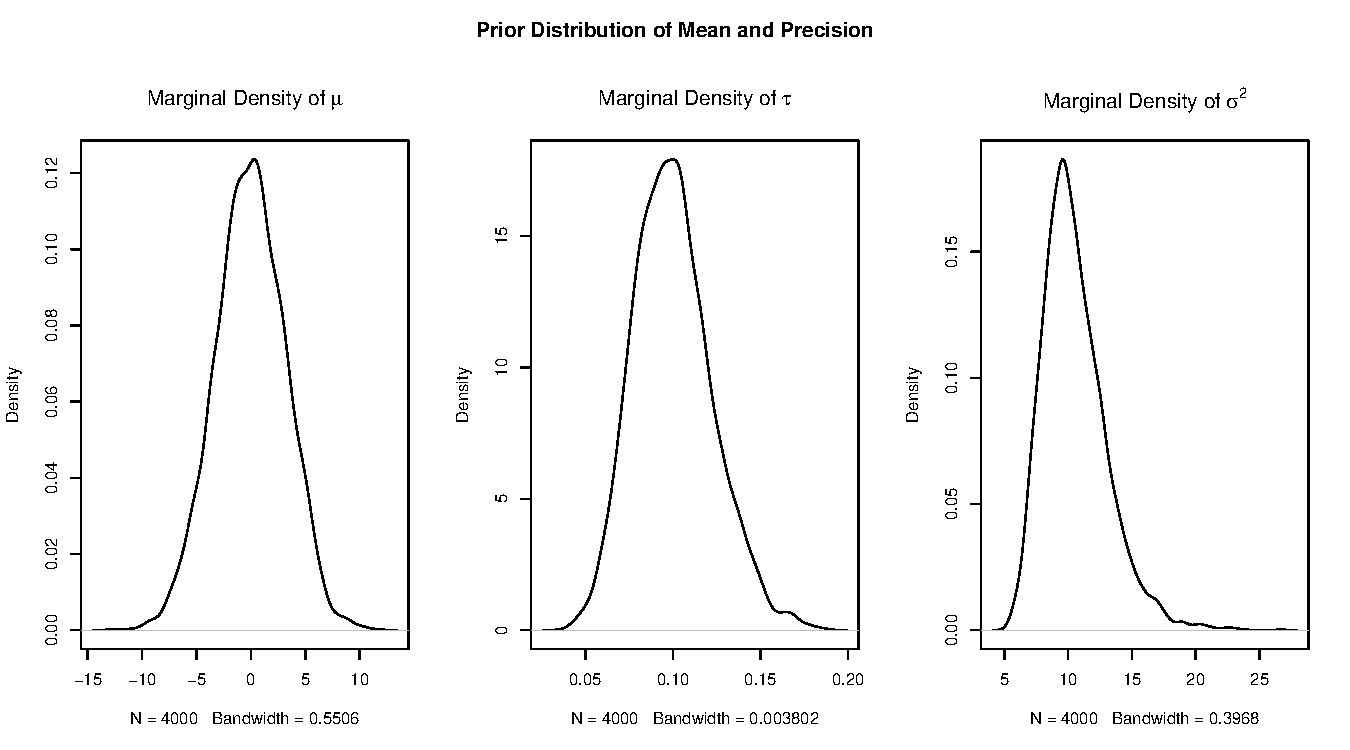
\includegraphics{03-lec_files/figure-latex/prior-sim-1} \end{center}

\hypertarget{implementing-the-gibbs-sampler-for-the-posterior}{%
\subsubsection{Implementing the Gibbs sampler for the posterior}\label{implementing-the-gibbs-sampler-for-the-posterior}}

Code: Gibbs sampler for the posterior

\begin{Shaded}
\begin{Highlighting}[]
\CommentTok{\# Define function}
\NormalTok{draw\_from\_posterior }\OtherTok{\textless{}{-}} \ControlFlowTok{function}\NormalTok{(theta,}
\NormalTok{                                omega,}
\NormalTok{                                alpha,}
\NormalTok{                                beta,}
\NormalTok{                                n\_warmup,}
\NormalTok{                                n\_draws,}
\NormalTok{                                data,}
                                \AttributeTok{seed =} \DecValTok{20210329}\NormalTok{,}
                                \AttributeTok{keep\_warmup =} \ConstantTok{TRUE}\NormalTok{) \{}
  \CommentTok{\# Set seed}
  \FunctionTok{set.seed}\NormalTok{(seed)}

  \CommentTok{\# Length of chain}
\NormalTok{  len\_chain }\OtherTok{\textless{}{-}}\NormalTok{ n\_warmup }\SpecialCharTok{+}\NormalTok{ n\_draws}
  
  \CommentTok{\# Data characteristics}
\NormalTok{  n\_data }\OtherTok{\textless{}{-}} \FunctionTok{length}\NormalTok{(data)  }
\NormalTok{  mean\_data }\OtherTok{\textless{}{-}} \FunctionTok{mean}\NormalTok{(data) }

  \CommentTok{\# Initialize containers}
\NormalTok{  mu }\OtherTok{\textless{}{-}} \FunctionTok{rep}\NormalTok{(}\ConstantTok{NA}\NormalTok{, len\_chain)}
\NormalTok{  tau }\OtherTok{\textless{}{-}} \FunctionTok{rep}\NormalTok{(}\ConstantTok{NA}\NormalTok{, len\_chain)}
  
  \CommentTok{\# Run Gibbs sampler}
  \ControlFlowTok{for}\NormalTok{ (i }\ControlFlowTok{in} \FunctionTok{seq\_len}\NormalTok{(len\_chain)) \{}
    \ControlFlowTok{if}\NormalTok{ (i }\SpecialCharTok{==} \DecValTok{1}\NormalTok{) \{}
      \DocumentationTok{\#\# Iteration 1: Initialize from prior}
\NormalTok{      alpha\_star }\OtherTok{\textless{}{-}}\NormalTok{ alpha}
\NormalTok{      beta\_star }\OtherTok{\textless{}{-}}\NormalTok{ beta}
\NormalTok{    \} }\ControlFlowTok{else}\NormalTok{ \{}
      \DocumentationTok{\#\# Iterations 2+: Update alpha and beta}
\NormalTok{      alpha\_star }\OtherTok{\textless{}{-}}\NormalTok{ alpha }\SpecialCharTok{+}\NormalTok{ n\_data }\SpecialCharTok{/} \DecValTok{2}
\NormalTok{      beta\_star }\OtherTok{\textless{}{-}}\NormalTok{ beta }\SpecialCharTok{+} \FunctionTok{sum}\NormalTok{(((data }\SpecialCharTok{{-}}\NormalTok{ mu[i }\SpecialCharTok{{-}} \DecValTok{1}\NormalTok{]) }\SpecialCharTok{\^{}} \DecValTok{2}\NormalTok{) }\SpecialCharTok{/} \DecValTok{2}\NormalTok{)}
\NormalTok{    \}}
    
    \DocumentationTok{\#\# Sample tau}
\NormalTok{    tau[i] }\OtherTok{\textless{}{-}} \FunctionTok{rgamma}\NormalTok{(}\DecValTok{1}\NormalTok{, alpha\_star, beta\_star)}
    
    \DocumentationTok{\#\# Update theta and omega}
\NormalTok{    theta\_star }\OtherTok{\textless{}{-}}
\NormalTok{      (omega }\SpecialCharTok{*}\NormalTok{ theta }\SpecialCharTok{+}\NormalTok{ n\_data }\SpecialCharTok{*}\NormalTok{ tau[i] }\SpecialCharTok{*}\NormalTok{ mean\_data) }\SpecialCharTok{/}
\NormalTok{      (omega }\SpecialCharTok{+}\NormalTok{ n\_data }\SpecialCharTok{*}\NormalTok{ tau[i])}
\NormalTok{    omega\_star }\OtherTok{\textless{}{-}}\NormalTok{ omega }\SpecialCharTok{+}\NormalTok{ n\_data }\SpecialCharTok{*}\NormalTok{ tau[i]}
    
    \DocumentationTok{\#\# Sample mu}
\NormalTok{    mu[i] }\OtherTok{\textless{}{-}} \FunctionTok{rnorm}\NormalTok{(}\DecValTok{1}\NormalTok{, theta\_star, }\DecValTok{1} \SpecialCharTok{/} \FunctionTok{sqrt}\NormalTok{(omega\_star))}
\NormalTok{  \}}
  
  \DocumentationTok{\#\# Conditionally discard warmup{-}draws}
  \ControlFlowTok{if}\NormalTok{ (}\SpecialCharTok{!}\NormalTok{keep\_warmup) \{}
\NormalTok{    tau }\OtherTok{\textless{}{-}}\NormalTok{ tau[(n\_warmup }\SpecialCharTok{+} \DecValTok{1}\NormalTok{)}\SpecialCharTok{:}\NormalTok{len\_chain]}
\NormalTok{    mu }\OtherTok{\textless{}{-}}\NormalTok{ mu[(n\_warmup }\SpecialCharTok{+} \DecValTok{1}\NormalTok{)}\SpecialCharTok{:}\NormalTok{len\_chain]}
\NormalTok{  \}}
  
  \DocumentationTok{\#\# Return output}
  \FunctionTok{return}\NormalTok{(}\FunctionTok{list}\NormalTok{(}\AttributeTok{mu =}\NormalTok{ mu,}
              \AttributeTok{tau =}\NormalTok{ tau))}
\NormalTok{\}}
\end{Highlighting}
\end{Shaded}

\begin{center}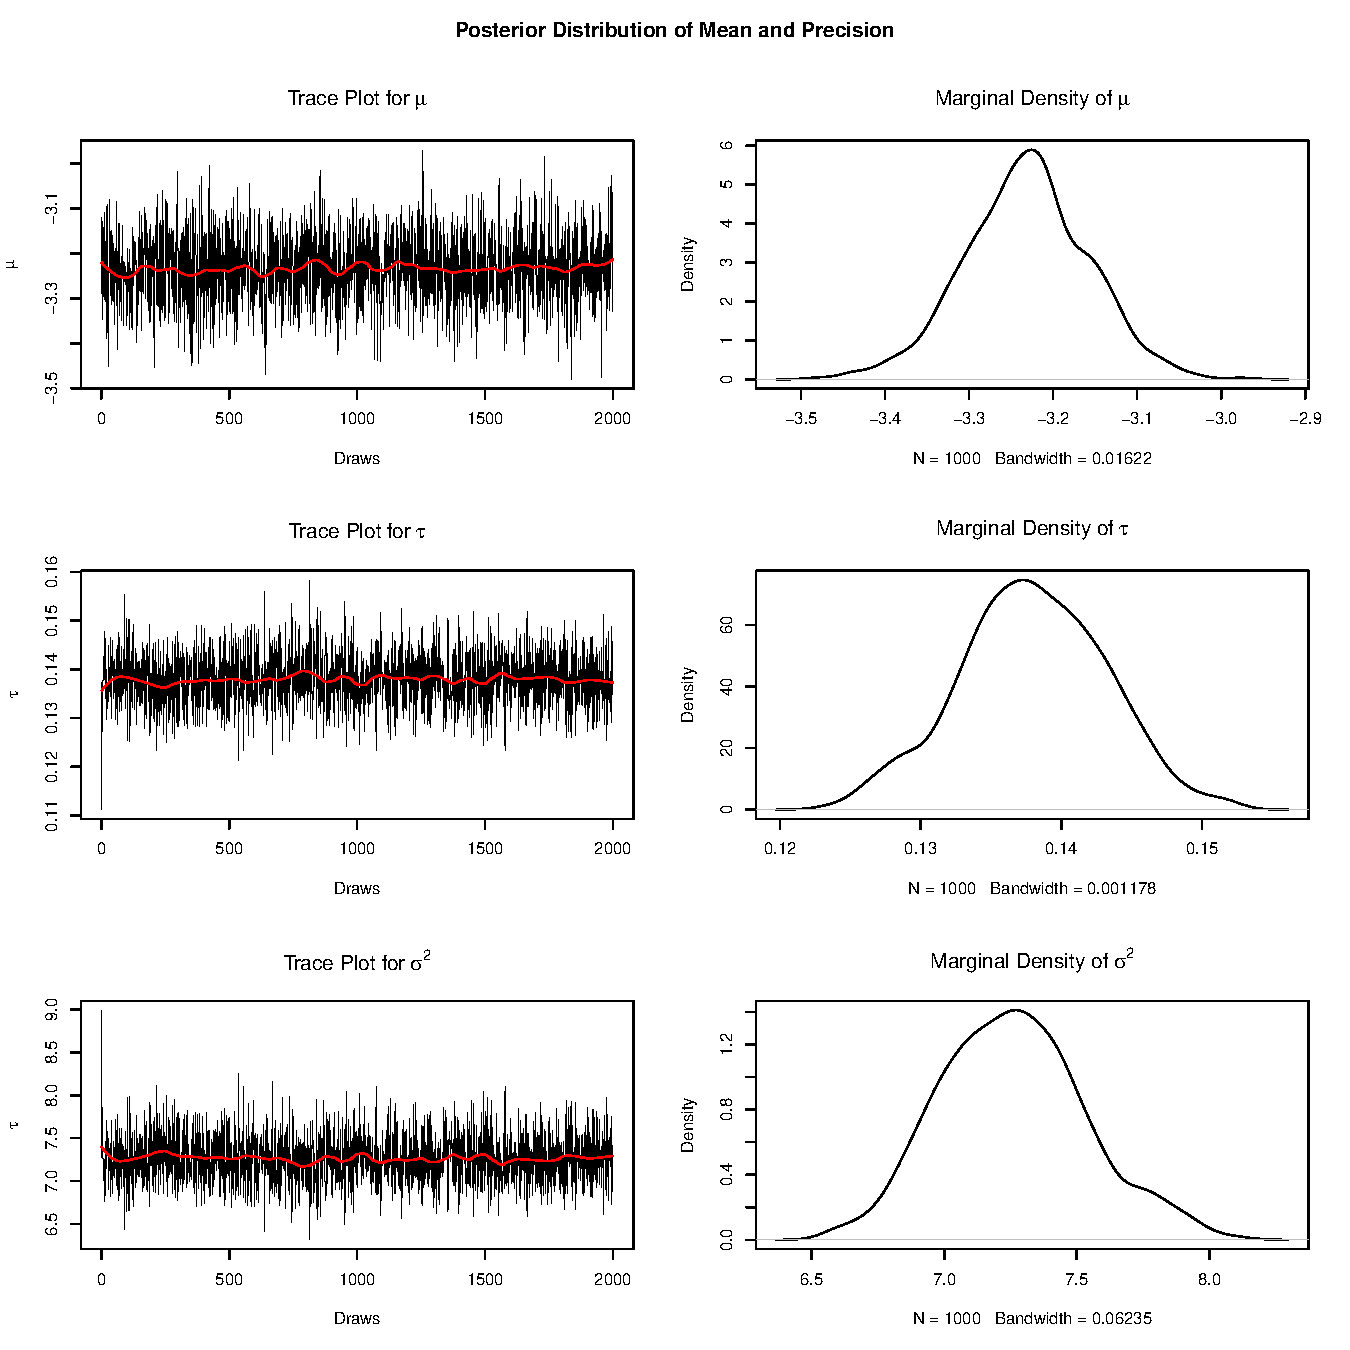
\includegraphics{03-lec_files/figure-latex/posterior-sim-1} \end{center}

\hypertarget{how-the-sampler-explores-the-joint-posterior-density}{%
\subsubsection{How the sampler explores the joint posterior density}\label{how-the-sampler-explores-the-joint-posterior-density}}

\begin{center}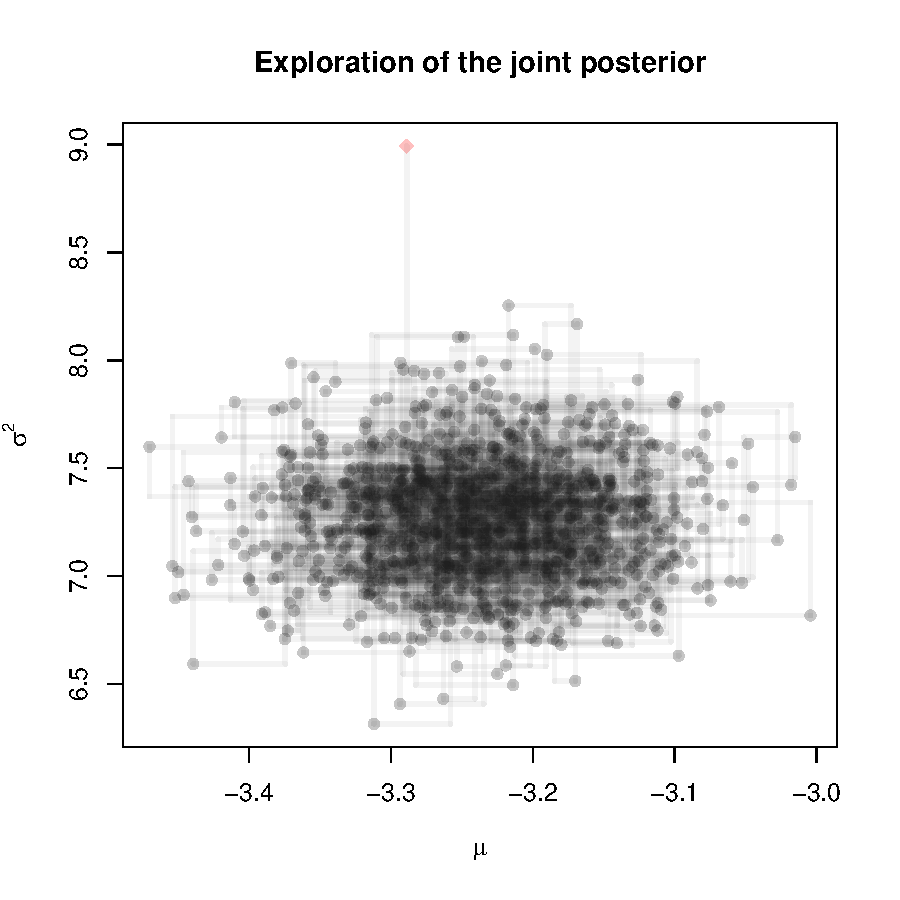
\includegraphics{03-lec_files/figure-latex/joint-posterior-1} \end{center}

\hypertarget{convergence-diagnostics}{%
\subsection{Convergence diagnostics}\label{convergence-diagnostics}}

\hypertarget{why-diagnose}{%
\subsubsection{Why diagnose?}\label{why-diagnose}}

MCMC algorithms use iterative algorithms to explore posterior distributions and to produce numerical approximations thereof.

However, even with appropriately specified models and algorithms, we can never know a priori if and when a chain has converged to its target distribution. We must thus rely on \emph{convergence diagnostics}.

\emph{Important:} Convergence diagnostics cannot show or prove convergence. They can only show signs of non-convergence!

To conclude that the post-warmup draws of our sampler in fact explore the target distribution, we want to show at least two things:

\begin{enumerate}
\def\labelenumi{\arabic{enumi}.}
\tightlist
\item
  Every chain is in a stationary state (i.e., does not ``wander off'' the target distribution)
\item
  Multiple independent chains are in the same stationary state (i.e., no convergence to different target distributions given identical data)
\end{enumerate}

\hypertarget{generic-diagnostics}{%
\subsubsection{Generic diagnostics}\label{generic-diagnostics}}

Generic diagnostics (see \href{https://www.routledge.com/Bayesian-Methods-A-Social-and-Behavioral-Sciences-Approach-Third-Edition/Gill/p/book/9781439862483}{Gill 2015, Ch. 14.3}) include:

\begin{enumerate}
\def\labelenumi{\arabic{enumi}.}
\tightlist
\item
  \textbf{Potential scale reduction statistic} \(\hat{R}\) (aka Gelman-Rubin convergence diagnostic)
  \[\small \widehat{Var}(\theta) = (1 - \frac{1}{\mathtt{n_{iter}}})
   \underbrace{\Bigg(\frac{1}{ \mathtt{n_{chains}} (\mathtt{n_{iter}} - 1)} \sum_{j=1}^{\mathtt{n_{chains}}} \sum_{i=1}^{\mathtt{n_{iter}}} (\theta_{ij} - \bar{\theta_j})^2 \Bigg)}_{\text{Within chain var}} + 
   \frac{1}{\mathtt{n_{iter}}}  \underbrace{\Bigg(\frac{\mathtt{n_{iter}}}{\mathtt{n_{chains} - 1}} \sum_{j=1}^{\mathtt{n_{chains}}} (\bar{\theta_j} - \bar{\bar{\theta}})^2\Bigg)}_{\text{Between chain var}}\]

  \begin{itemize}
  \tightlist
  \item
    low values indicate that chains are stationary (convergence to target distribution within chains)
  \item
    low values indicate that chains mix (convergence to same target distribution across chains)
  \end{itemize}
\item
  \textbf{Geweke Time-Series Diagnostic}: Compare non-overlapping post-warmup portions of each chain to test within-convergence
\item
  \textbf{Heidelberger and Welch Diagnostic}: Compare early post-warmup portion of each chain with late portion to test within-convergence
\item
  \textbf{Raftery and Lewis Integrated Diagnostic}: Evaluates the full chain of a pilot run (requires that \texttt{save\_warmup\ =\ TRUE}) to estimate minimum required length of warmup and sampling
\end{enumerate}

These are implemented as part of the \texttt{coda} package (Output Analysis and Diagnostics for MCMC).

\hypertarget{visual-diagnostics}{%
\subsubsection{Visual diagnostics}\label{visual-diagnostics}}

The most widespread visual diagnostics are:

\begin{enumerate}
\def\labelenumi{\arabic{enumi}.}
\tightlist
\item
  \textbf{Traceplots}: Visually inspect if chains are stationary and have converged to the same distribution
\item
  \textbf{Autocorrelation plots}: Visually inspect if the chain is sluggish in exploring the parameter space.
\end{enumerate}

\hypertarget{application-1}{%
\subsubsection{Application}\label{application-1}}

In the following, we will use multiple chain runs of our sampler in conjunction with the \texttt{coda} package to check for signs of non-convergence.

Note that \texttt{coda} functions require that we combine our chains into \texttt{mcmc.list} objects.

\hypertarget{raftery-and-lewis-integrated-diagnostic}{%
\subsubsection{Raftery and Lewis Integrated Diagnostic}\label{raftery-and-lewis-integrated-diagnostic}}

The Raftery-Lewis diagnostic takes a single chain, including warm-up draws, to estimate the minimum required length of warmup and sampling runs:

\begin{verbatim}
## 
## Quantile (q) = 0.5
## Accuracy (r) = +/- 0.0125
## Probability (s) = 0.95 
##                                            
##      Burn-in  Total Lower bound  Dependence
##      (M)      (N)   (Nmin)       factor (I)
##  mu  2        6278  6147         1.020     
##  tau 2        5906  6147         0.961
\end{verbatim}

\hypertarget{gelman-rubin-geweke-and-heidelberger-welch-diagnostics}{%
\subsubsection{Gelman-Rubin, Geweke, and Heidelberger-Welch diagnostics}\label{gelman-rubin-geweke-and-heidelberger-welch-diagnostics}}

We will use the recommended run-length from the Raftery-Lewis diagnostic for
four independent runs of our sampler.

We will ensure that ou chains run independently (i.e., using different starting values and different random number sequences) by setting different seed:

\begin{Shaded}
\begin{Highlighting}[]
\NormalTok{seeds }\OtherTok{\textless{}{-}} \FunctionTok{sample}\NormalTok{(}\DecValTok{10001}\SpecialCharTok{:}\DecValTok{99999}\NormalTok{, }\DecValTok{4}\NormalTok{)}
\NormalTok{draws\_multiple\_chains }\OtherTok{\textless{}{-}} \FunctionTok{lapply}\NormalTok{(seeds,}
                                \ControlFlowTok{function}\NormalTok{(seed) \{}
                                  \FunctionTok{as.mcmc}\NormalTok{(}\FunctionTok{simplify2array}\NormalTok{(}
                                    \FunctionTok{draw\_from\_posterior}\NormalTok{(}
                                      \AttributeTok{theta =} \DecValTok{0}\NormalTok{,}
                                      \AttributeTok{omega =}\NormalTok{ .}\DecValTok{1}\NormalTok{,}
                                      \AttributeTok{alpha =} \DecValTok{20}\NormalTok{,}
                                      \AttributeTok{beta =} \DecValTok{200}\NormalTok{,}
                                      \AttributeTok{n\_warmup =} \DecValTok{200}\NormalTok{,}
                                      \AttributeTok{n\_draws =} \DecValTok{6147}\NormalTok{,}
                                      \AttributeTok{data =}\NormalTok{ gles}\SpecialCharTok{$}\NormalTok{sup\_afd,}
                                      \AttributeTok{keep\_warmup =} \ConstantTok{FALSE}\NormalTok{,}
                                      \AttributeTok{seed =}\NormalTok{ seed}
\NormalTok{                                    )}
\NormalTok{                                  ))}
\NormalTok{                                \})}

\CommentTok{\# Save as mcmc.list}
\NormalTok{draws\_multiple\_chains }\OtherTok{\textless{}{-}} \FunctionTok{as.mcmc.list}\NormalTok{(draws\_multiple\_chains)}
\end{Highlighting}
\end{Shaded}

\begin{verbatim}
## Potential scale reduction factors:
## 
##     Point est. Upper C.I.
## mu           1          1
## tau          1          1
## 
## Multivariate psrf
## 
## 1
\end{verbatim}

\begin{verbatim}
## [[1]]
## 
## Fraction in 1st window = 0.1
## Fraction in 2nd window = 0.5 
## 
##     mu    tau 
## 0.9199 0.7017 
## 
## 
## [[2]]
## 
## Fraction in 1st window = 0.1
## Fraction in 2nd window = 0.5 
## 
##      mu     tau 
## -0.1502  0.2656 
## 
## 
## [[3]]
## 
## Fraction in 1st window = 0.1
## Fraction in 2nd window = 0.5 
## 
##      mu     tau 
## -0.1191 -0.9184 
## 
## 
## [[4]]
## 
## Fraction in 1st window = 0.1
## Fraction in 2nd window = 0.5 
## 
##    mu   tau 
## 1.194 1.114
\end{verbatim}

\begin{verbatim}
## [[1]]
##                                   
##     Stationarity start     p-value
##     test         iteration        
## mu  passed       1         0.204  
## tau passed       1         0.695  
##                               
##     Halfwidth Mean   Halfwidth
##     test                      
## mu  passed    -3.231 0.00182  
## tau passed     0.138 0.00013  
## 
## [[2]]
##                                   
##     Stationarity start     p-value
##     test         iteration        
## mu  passed       1         0.771  
## tau passed       1         0.332  
##                               
##     Halfwidth Mean   Halfwidth
##     test                      
## mu  passed    -3.230 0.001855 
## tau passed     0.138 0.000134 
## 
## [[3]]
##                                   
##     Stationarity start     p-value
##     test         iteration        
## mu  passed       1         0.388  
## tau passed       1         0.552  
##                               
##     Halfwidth Mean   Halfwidth
##     test                      
## mu  passed    -3.230 0.001855 
## tau passed     0.138 0.000132 
## 
## [[4]]
##                                   
##     Stationarity start     p-value
##     test         iteration        
## mu  passed       1         0.652  
## tau passed       1         0.340  
##                               
##     Halfwidth Mean   Halfwidth
##     test                      
## mu  passed    -3.229 0.00186  
## tau passed     0.138 0.00014
\end{verbatim}

\hypertarget{trace-plots}{%
\subsubsection{Trace plots}\label{trace-plots}}

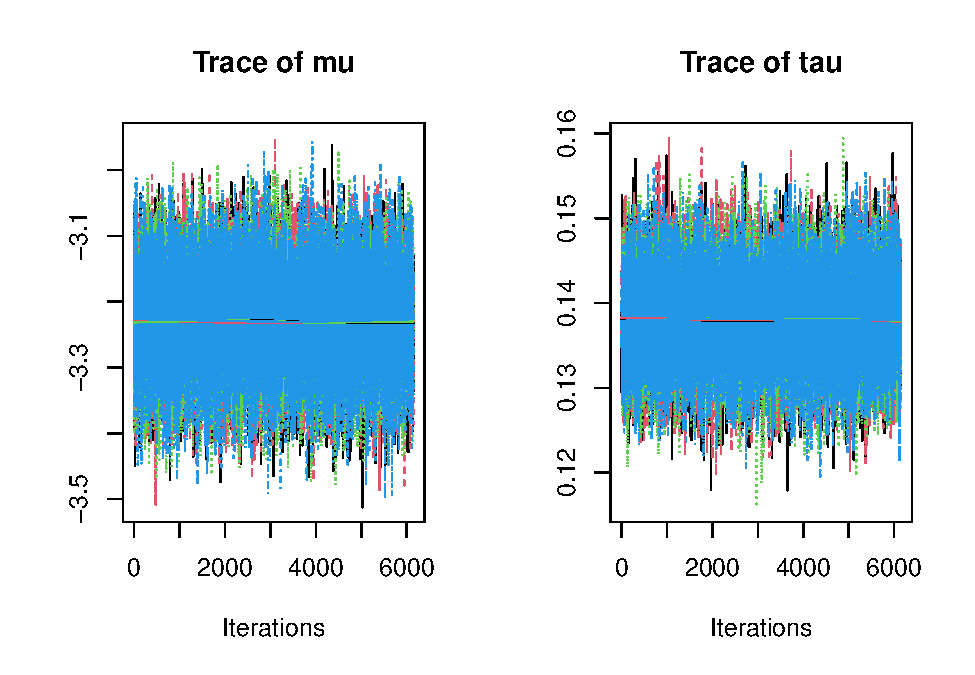
\includegraphics{03-lec_files/figure-latex/trace-1.pdf}

\hypertarget{autocorrelation-plots}{%
\subsubsection{Autocorrelation plots}\label{autocorrelation-plots}}

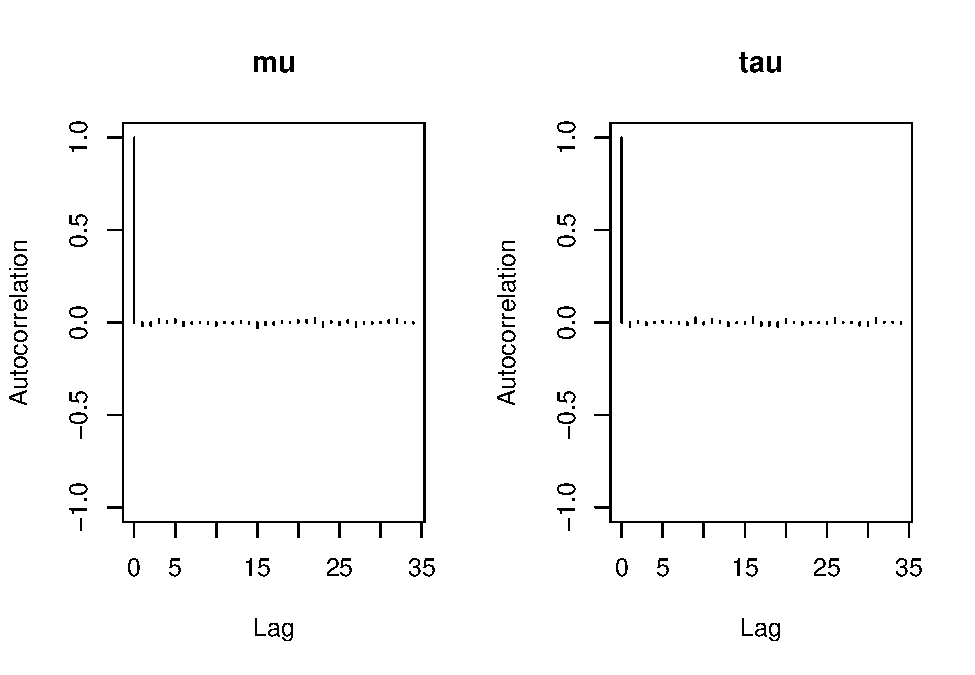
\includegraphics{03-lec_files/figure-latex/autocorr-1.pdf} 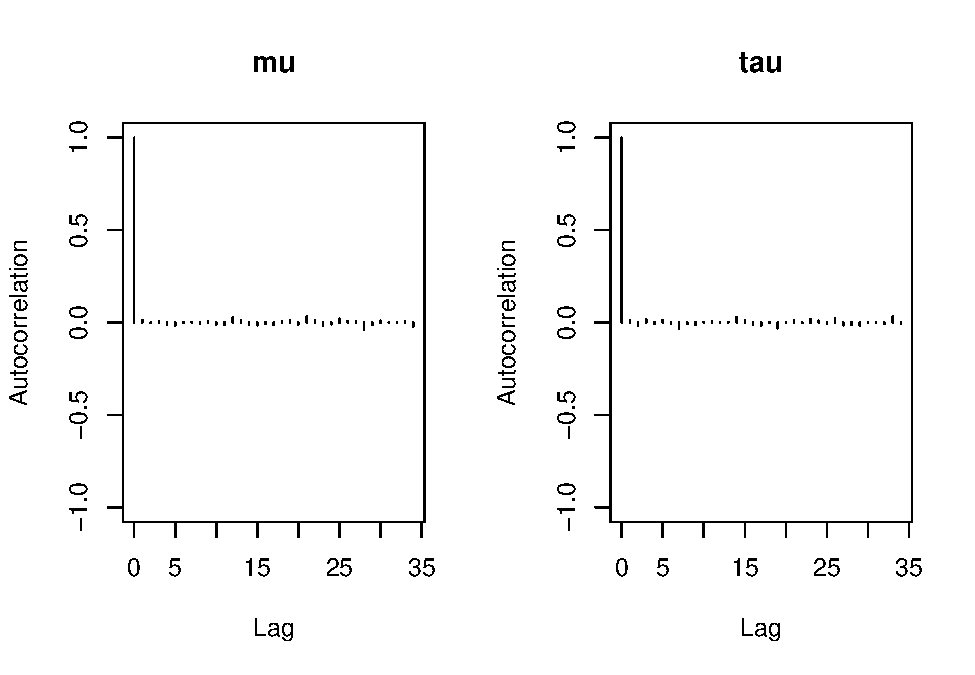
\includegraphics{03-lec_files/figure-latex/autocorr-2.pdf} 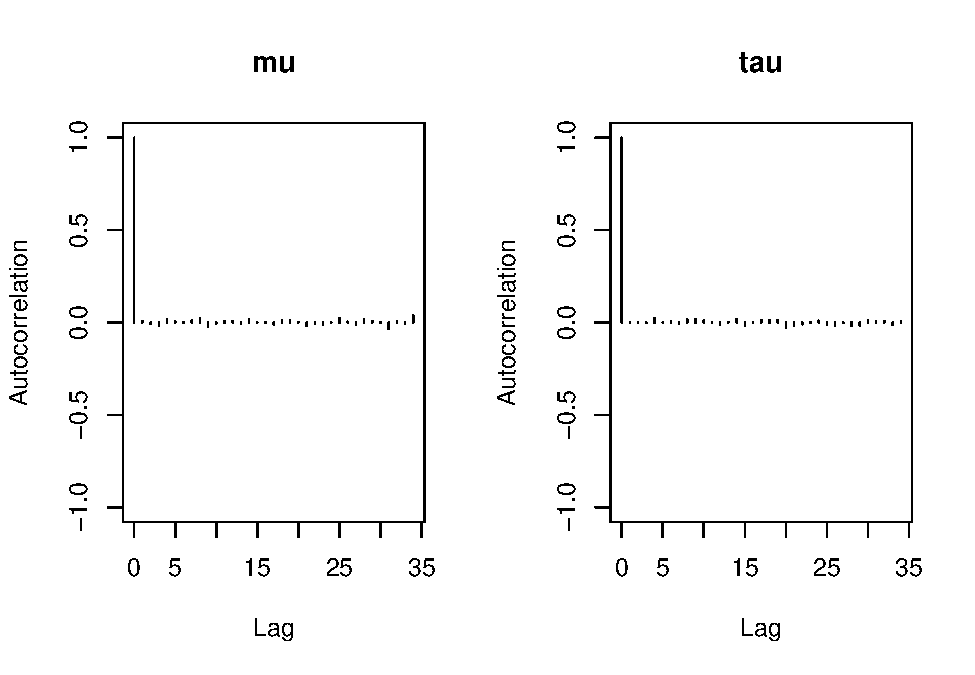
\includegraphics{03-lec_files/figure-latex/autocorr-3.pdf} 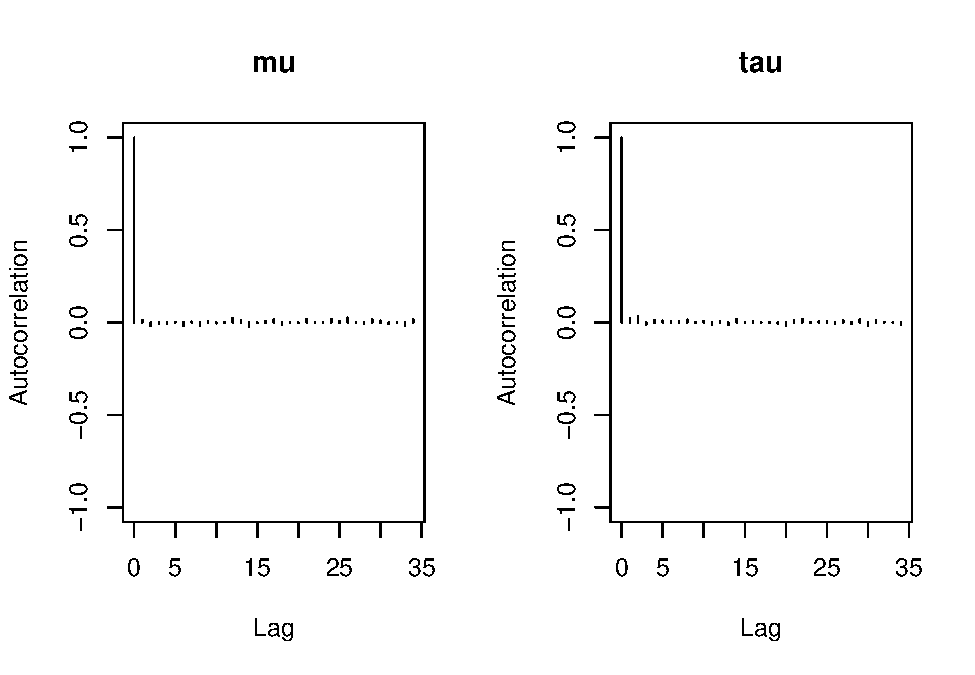
\includegraphics{03-lec_files/figure-latex/autocorr-4.pdf}

\hypertarget{contrasting-bayesian-and-frequentist-approaches}{%
\subsection{Contrasting Bayesian and frequentist approaches}\label{contrasting-bayesian-and-frequentist-approaches}}

\hypertarget{priors}{%
\subsubsection{Priors}\label{priors}}

\begin{itemize}
\tightlist
\item
  Choice of priors allows us to explicitly incorporate prior beliefs about parameters\ldots{}
\item
  \ldots but also comes with the obligation to be transparent and responsible with respect to the subjectivity this brings into our analyses
\end{itemize}

\hypertarget{inference}{%
\subsubsection{Inference}\label{inference}}

\hypertarget{interpretation}{%
\paragraph{Interpretation}\label{interpretation}}

\begin{itemize}
\tightlist
\item
  Bayesian inference does note presume large (quasi-infinite) streams of independent identically distributed (IID) data; data are considered fixed, parameters random.
\item
  This allows for straightforward interpretations of inferential uncertainty:

  \begin{itemize}
  \tightlist
  \item
    \emph{Bayesian}: ``Given the data, we can conclude that there is a 95\% probability that the mean is between 8 and 12, with highest probability density at a value of 10''.
  \item
    \emph{Frequentist}: ``If we took a large number of independent random samples from the same population and constructed a 95\% confidence interval around the sample for each of them, these confidence intervals would contain the \emph{true} population mean 95\% of the time. Given this long-run frequency, we are 95\% confident that the specific 95\% confidence intervals from our singular sample contains the true population parameter\ldots{}''.
  \end{itemize}
\end{itemize}

\hypertarget{finite-sample-and-asymptotic-properties}{%
\paragraph{Finite-sample and asymptotic properties}\label{finite-sample-and-asymptotic-properties}}

\begin{itemize}
\tightlist
\item
  Bayesian inference allows for exact inference in finite-sample applications where the asymptotic properties of MLE estimators are implausible (normal approximation, etc.)\ldots{}
\item
  \ldots yet, posterior distribution often asymptotically converge to the sampling distribution of MLE estimators (\href{https://en.wikipedia.org/wiki/Bernstein\%E2\%80\%93von_Mises_theorem}{Bernstein-von-Mises Theorem})
\end{itemize}

\hypertarget{flexibility-and-computational-reliability}{%
\subsubsection{Flexibility and computational reliability}\label{flexibility-and-computational-reliability}}

\begin{itemize}
\tightlist
\item
  The use of MCMC algorithms for probabilistic approximate inference makes Bayesian approaches incredibly flexible and allows for computationally reliable estimation of complex, analytically intractable marginal likelihoods (avoids integration of super high-dimensional integrals)\ldots{}
\item
  \ldots but sometimes comes with the necessity of high computational resources and/or long computation times, and always necessitates convergence diagnosis and model checking
\end{itemize}

\end{document}
